\documentclass[iicol,Numbered]{sn-jnl}

\usepackage{amsmath,amssymb,amsfonts}
\usepackage{graphicx}
\graphicspath{{./}{./figures/}}
\usepackage{booktabs}
\usepackage{tabularx}
\usepackage{array}
\usepackage{multirow}
\usepackage{enumitem}
\usepackage{xcolor}
\usepackage{algorithm}
\usepackage{algpseudocode}
\usepackage{url}
\usepackage{microtype}
\usepackage{makecell}
\usepackage{ragged2e}
\usepackage{placeins}
\usepackage{manyfoot}

\newcolumntype{P}[1]{>{\RaggedRight\arraybackslash}p{#1}}
\newcolumntype{Y}{>{\RaggedRight\arraybackslash}X}
\newcolumntype{C}{>{\centering\arraybackslash}X}
\renewcommand{\arraystretch}{1.15}
\setlength{\textfloatsep}{5pt plus 1pt minus 1pt}
\setlength{\floatsep}{5pt plus 1pt minus 1pt}
\setlength{\intextsep}{5pt plus 1pt minus 1pt}
\setlength{\abovecaptionskip}{2pt}
\setlength{\belowcaptionskip}{0pt}
\setlength{\emergencystretch}{2em}
\setlength{\abovedisplayskip}{4pt plus 1pt minus 1pt}
\setlength{\belowdisplayskip}{4pt plus 1pt minus 1pt}
\setlength{\abovedisplayshortskip}{2pt plus 1pt minus 1pt}
\setlength{\belowdisplayshortskip}{2pt plus 1pt minus 1pt}
\setlist{nosep,topsep=2pt,parsep=0pt,partopsep=0pt}
\setlength{\tabcolsep}{2.8pt}
\renewcommand{\arraystretch}{1.02}
\raggedbottom
\sloppy

\begin{document}

\title[FedZT-Edge]{FedZT-Edge: A Federated, Zero-Trust, WebAssembly-Based
Intrusion Detection Framework for Resource-Constrained Edge Networks}

\author[1]{\fnm{Mohid} \sur{Abbas}}\email{i240074@isb.nu.edu.pk}
\author[1]{\fnm{Ali} \sur{Khan}}\email{i240069@isb.nu.edu.pk}

\affil[1]{\orgdiv{Department of Computer Science}, \orgname{FAST-NUCES}, \orgaddress{\street{H-11/4},
\city{Islamabad}, \country{Pakistan}}}

\abstract{Edge devices in industrial and smart-city deployments face a growing
range of network intrusions, yet their limited compute makes centralised
detection hard to justify. This paper presents FedZT-Edge, a framework that
combines federated learning, zero-trust access control and WebAssembly (Wasm)
sandboxing so that intrusion detection can run at the edge without pooling raw
traffic. Aggregation uses FedProx ($\mu=0.1$) to cope with non-IID traffic. A
two-stage norm-ratio and GMM filter screens gradient updates, AES-256-GCM and
RSA-2048 protect model transfers, and a static-threshold trust policy is
evaluated next to an undertrained DQN. The headline scores use the
static-threshold policy. On UNSW-NB15 and CICIDS-2017 (10 clients, Dirichlet
$\alpha=0.5$, seeds $[42,101,2024]$), FedZT-Edge reaches macro-F1 of
$0.841\pm0.020$ and $0.915\pm0.006$, in line with plain FedProx, and all raw
traffic stays on the clients. It improves on the isolated local baseline by
34.4 and 35.4 percentage points. On CICIDS-2017 the gaps to the centralised and
IID FedAvg baselines are significant after Holm correction ($p<0.05$); on
UNSW-NB15 no comparison is significant with three seeds. Under the actual
$\alpha=0.5$ conditions the UNSW-NB15 filter has zero recall at 20 to 30\%
attack, and the DQN underperforms the static rule. Encryption adds 0.616\,ms
per measured round operation, and Wasm batch inference takes 0.375\,ms on a
laptop-class host.}

\keywords{federated learning, intrusion detection, zero-trust, WebAssembly, edge computing}

\maketitle
\setcounter{page}{1}

\section{Introduction}\label{sec:intro}

Edge computing has put real processing power into IoT gateways, industrial
sensors and smart-city infrastructure, and it has widened the attack surface at
the same time. Edge nodes have little memory and power, often sit behind
unreliable uplinks, and can be within physical reach of an attacker. Sending raw
network traffic to a central server for analysis consumes bandwidth and raises
data-residency problems~\cite{mcmahan2017,li2020federated}.

Federated learning (FL) avoids moving the data: clients train locally and share
only model updates~\cite{mcmahan2017}. Two difficulties remain. FedAvg copes
poorly with non-IID client data, which is the normal case in heterogeneous edge
fleets. The aggregation server also becomes a point of trust, since a few
compromised clients can poison the global model by flipping labels or
manipulating gradients, often unnoticed~\cite{tolpegin2020,bagdasaryan2020}.
Zero-trust architecture~\cite{nist2020} treats every participant as untrusted
until verified, which suits this problem, yet its combination with federated
IDS has received little attention~\cite{chen2021zero}. WebAssembly adds a third
element: running inference in a Wasm sandbox isolates it from the rest of the
edge OS and limits the damage if the model is compromised~\cite{haas2017wasm}.

This paper addresses three gaps. \textbf{G1}: an IDS pipeline that keeps raw
traffic local while combining federated training with edge deployment.
\textbf{G2}: evaluation of poisoning robustness under non-IID client
partitions. \textbf{G3}: evidence on running federated IDS inference inside a
Wasm sandbox on constrained hardware. G2 and G3 are only partly closed. The
filter fails at high attack rates in the tested non-IID setting, and Wasm was
measured on a laptop rather than dedicated edge hardware.

FedZT-Edge combines these elements in one pipeline. The contributions are:

\begin{enumerate}[leftmargin=*,itemsep=3pt]
\item A FedProx-based federated IDS that reaches macro-F1 of 0.841 on
      UNSW-NB15 and 0.915 on CICIDS-2017 under non-IID partitioning
      ($\alpha=0.5$) without exchanging raw traffic.
\item A two-stage update filter that combines a norm-ratio test with a
      two-component Gaussian mixture model (GMM) over update norms and pairwise
      cosine distances, evaluated under label flipping at four
      malicious-client rates.
\item A DQN-based zero-trust policy engine with a preliminary evaluation. The
      undertrained DQN currently performs worse than a static threshold rule.
\item A Wasm-sandboxed inference module with 0.375\,ms batch latency and
      0.616\,ms cryptographic overhead, measured on a laptop-class host.
\item An ablation over eight design axes on both datasets, with
      Holm-corrected pairwise tests over three seeds.
\end{enumerate}

Section~\ref{sec:related} reviews related work, Section~\ref{sec:method}
describes the design, and Section~\ref{sec:setup} gives the experimental setup.
Results are in Section~\ref{sec:results}, the comparison with prior work in
Section~\ref{sec:comparison}, and the ablation in Section~\ref{sec:ablation}.
Section~\ref{sec:discussion} covers limitations, and
Section~\ref{sec:conclusion} concludes with future work.

\section{Related Work}\label{sec:related}

\subsection{Federated Learning for Intrusion Detection}

FedAvg~\cite{mcmahan2017} set the basic FL training protocol but was designed
and tested on IID data. Li et al.~\cite{li2020federated} added a proximal term
(FedProx) that keeps local models near the global checkpoint and improves
convergence when client distributions differ. Nguyen et al.~\cite{nguyen2019}
applied FL to IoT anomaly detection and found that privacy need not cost
detection accuracy, although their clients held similar amounts of similar
data. Hozouri et al.~\cite{hozouri2023} report that strong skew
($\alpha<0.2$) can cost up to 20 percentage points of macro-F1, which motivates
the heterogeneity sweep in Section~\ref{sec:results}.

\subsection{Adversarial Robustness in Federated Systems}

Tolpegin et al.~\cite{tolpegin2020} studied label-flipping attacks on FL and
showed that one malicious client in ten can noticeably degrade the global model.
Bagdasaryan et al.~\cite{bagdasaryan2020} showed that a single compromised
client can replace the global model in one round with a suitably scaled update.
FLTrust~\cite{cao2021fltrust} stays robust up to 30\% malicious clients by
anchoring aggregation to a small clean dataset on the server. That requires
labelled data on the server, which weakens the privacy model that motivates
federated IDS. Karunamurthy et al.~\cite{karunamurthy2023} cluster gradient
updates with K-Means to find outliers and report good results at low attack
rates, with precision dropping once attackers dominate.

\subsection{Zero-Trust and WebAssembly at the Edge}

NIST SP\,800-207~\cite{nist2020} defines the policy decision point (PDP) and
policy enforcement point (PEP) model used by zero-trust systems. Chen et
al.~\cite{chen2021zero} applied it to IoT gateways, updating a per-device trust
score after every request, and saw less lateral movement in controlled tests.
On the Wasm side, Haas et al.~\cite{haas2017wasm} introduced the bytecode format
and its security model. Weber et al.~\cite{weber2024} measured sub-millisecond
inference on microcontroller-class hardware; the hardware differs from the
laptop used here, so the numbers are context only. Djemaa et
al.~\cite{djemaa2022} and Zhang et al.~\cite{zhang2023} report 20 to 30\%
overhead over native execution for ML workloads, below the 25 to 56\% measured
here.

\subsection{Feature Selection and Centralised IDS Baselines}

Mahida~\cite{mahida2022} applied chi-square feature selection to UNSW-NB15 and
trained a centralised MLP to above 95\% accuracy. Albogami et
al.~\cite{albogami2023} reached macro-F1 above 0.96 on CICIDS-2017 with a
centralised deep network. These figures serve as ceilings for non-federated
training on the two benchmarks, so the gap to FedZT-Edge shows what the privacy
and security constraints cost.

\subsection{Positioning of FedZT-Edge}

Table~\ref{tab:related} summarises the prior work. The authors know of no
existing system that combines FL, zero-trust policy enforcement and Wasm
sandboxing and evaluates it with a full ablation on two standard network IDS
benchmarks. FedZT-Edge gives up some accuracy relative to centralised methods
and some robustness relative to FLTrust in return.

\begin{table*}[t]
\centering
\footnotesize
\caption{Summary of related work. FL: federated learning; ZT: zero-trust;
Wasm: WebAssembly. F1 is macro-F1; Acc is accuracy.}
\label{tab:related}
\setlength{\tabcolsep}{3pt}
\begin{tabularx}{\textwidth}{@{}P{2.9cm} Y Y Y Y Y@{}}
\toprule
\textbf{Study} & \textbf{Problem} & \textbf{Method} & \textbf{Dataset} &
\textbf{Key result} & \textbf{Limitation} \\
\midrule
McMahan et al.~\cite{mcmahan2017} & Private distributed training & FedAvg & MNIST, Shakespeare & Strong IID accuracy & Degrades under non-IID \\
Li et al.~\cite{li2020federated} & Non-IID convergence & FedProx & MNIST, FEMNIST, Shakespeare & Convergence guarantee & No security layer \\
Tolpegin et al.~\cite{tolpegin2020} & FL poisoning analysis & Label-flip study & MNIST, KDD99 & F1 collapses at 30\% attack & No full defence \\
Cao et al.~\cite{cao2021fltrust} & Robust aggregation & FLTrust (server anchor) & MNIST, CIFAR-10 & Original-paper result; not this study's UNSW-NB15 result & Needs labelled server data \\
Nguyen et al.~\cite{nguyen2019} & Federated IoT anomaly detection & FedAvg + CNN & N-BaIoT & High detection accuracy & IID partitioning \\
Mahida~\cite{mahida2022} & Network IDS & Chi-sq + MLP & UNSW-NB15 & Acc\,$>$\,95\% & Centralised \\
Albogami et al.~\cite{albogami2023} & Deep-learning IDS & DNN & CICIDS-2017 & F1\,$>$\,0.96 & Centralised \\
Hozouri et al.~\cite{hozouri2023} & Federated anomaly detection & FL + clustering & Custom network data & Good under mild non-IID & Severe skew not tested \\
Chen et al.~\cite{chen2021zero} & Zero-trust IoT gateway & Per-device trust score & Custom IoT traces & Less lateral movement & No FL \\
Weber et al.~\cite{weber2024} & Wasm on edge hardware & Runtime benchmark & Synthetic ML workload & Sub-ms inference & No IDS, no FL \\
Djemaa et al.~\cite{djemaa2022} & Wasm security overhead & Sandbox comparison & Synthetic & 20--30\% overhead & No IDS context \\
Karunamurthy et al.~\cite{karunamurthy2023} & Clustering-based FL defence & K-Means filter & MNIST & High precision at low attack rates & Precision drops at high rates \\
\midrule
\textbf{FedZT-Edge (this work)} & Federated ZT Wasm IDS & FedProx + GMM filter + DRL + Wasm & UNSW-NB15, CICIDS-2017 & F1\,=\,0.841 / 0.915 & DQN undertrained; Wasm on laptop \\
\bottomrule
\end{tabularx}
\end{table*}

\section{Proposed Methodology}\label{sec:method}

\subsection{Problem Formulation}

The system has $K=10$ edge clients. Client $k$ holds a private dataset
$\mathcal{D}_k=\{(\mathbf{x}_i,y_i)\}_{i=1}^{n_k}$ with
$\mathbf{x}_i\in\mathbb{R}^{20}$ a traffic feature vector and $y_i\in\{0,1\}$ a
binary label (normal or attack). The global objective is
\begin{equation}
\begin{aligned}
\min_{\mathbf{w}}\quad F(\mathbf{w})
 &=\sum_{k=1}^{K}\frac{n_k}{n}F_k(\mathbf{w}),\\
F_k(\mathbf{w})
 &=\frac{1}{n_k}\sum_{(\mathbf{x},y)\in\mathcal{D}_k}
   \ell\bigl(f(\mathbf{x};\mathbf{w}),y\bigr).
\end{aligned}
\label{eq:objective}
\end{equation}
where $n=\sum_k n_k$, $f(\cdot;\mathbf{w})$ is an MLP with shared weights
$\mathbf{w}$, and $\ell$ is the cross-entropy loss
\begin{equation}
\ell(\hat{y},y)=-\bigl[y\log\hat{y}+(1-y)\log(1-\hat{y})\bigr].
\label{eq:loss}
\end{equation}
No raw sample leaves the client that owns it. The model-export and conversion
toolchain used to produce the Wasm module is not recorded in the run notes and
remains to be documented.

\begin{figure*}[!t]
\centering
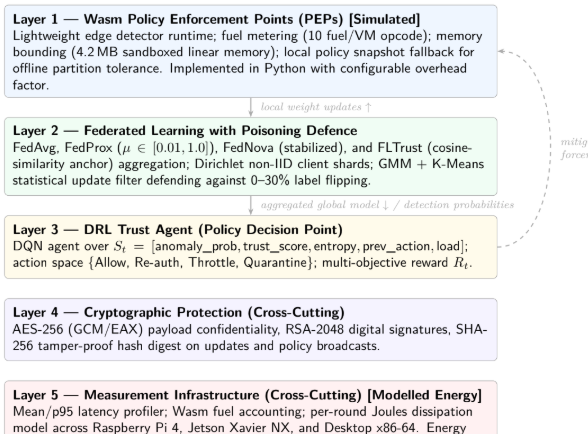
\includegraphics[width=0.96\textwidth,height=0.72\textheight,keepaspectratio]{architecture.png}
\caption{The five-layer FedZT-Edge architecture.}
\label{fig:architecture}
\end{figure*}

\subsection{System Architecture}

The system has five cooperating layers, shown in Figure~\ref{fig:architecture}.
Wasm policy enforcement points provide the edge runtime. Federated learning and
poisoning defence form the training layer. The DRL trust agent selects policy
actions, cryptographic protection secures exchanges between layers, and the
measurement infrastructure records latency and energy costs.

\textbf{Edge inference layer.} Each client runs a small MLP
(20\,$\to$\,32\,$\to$\,16\,$\to$\,2, ReLU, 1,234 parameters with biases) inside
the Wasmtime runtime~\cite{wasmtime2023}. The 20 input features are the top
chi-square-ranked traffic statistics, selected on the training partition only,
so the test set does not influence the choice.

\textbf{Cryptographic envelope.} Before sending an update, a client encrypts it
with AES-256-GCM for confidentiality and signs it with RSA-2048 for
authenticity. The server checks the signature before the update reaches
aggregation. On UNSW-NB15 this step costs 0.616\,ms per round.

\textbf{Federated aggregation layer.} The server aggregates verified updates
with FedProx, whose local objective adds a proximal term that limits client
drift:
\begin{equation}
\min_{\mathbf{w}_k}\; F_k(\mathbf{w}_k)+\frac{\mu}{2}\|\mathbf{w}_k-\mathbf{w}^t\|^2,
\label{eq:fedprox}
\end{equation}
with $\mathbf{w}^t$ the global model at round $t$ and $\mu=0.1$. Each update
$\Delta_k=\mathbf{w}_k-\mathbf{w}^t$ passes through the filter in
Section~\ref{sec:filter} before weighted averaging.

\textbf{Zero-trust policy layer.} A DQN agent keeps a trust vector
$\mathbf{z}\in[0,1]^K$ over the clients. In every round it observes a state
$s_t$ built from filter anomaly scores, each client's recent accuracy and its
communication latency, and picks one of four actions per client: full trust,
reduced weight, quarantine or eviction. If the central PDP cannot be reached,
clients use the most recent cached policy snapshot.

\textbf{Measurement infrastructure.} The evaluation records mean and
95th-percentile latency, Wasm fuel consumption and per-round energy estimates.
Results are reported separately for Raspberry Pi 4, Jetson Xavier NX and desktop
x86-64 hardware where measurements exist. Energy values are labelled as modelled
when they are not direct hardware measurements.

\subsection{Two-Stage Update Filter}\label{sec:filter}

Algorithm~\ref{alg:filter} gives the procedure.

\begin{algorithm}[t]
\caption{Two-stage norm-ratio and GMM update filter}
\label{alg:filter}
\begin{algorithmic}[1]
\Require Updates $\{\Delta_k\}_{k=1}^{K}$
\Statex \hspace{\algorithmicindent}Parameters: $\tau_{\mathrm{nr}}=4$, $\delta=0.4$, $\rho=0.3$
\State Compute $r_k=\|\Delta_k\|/\bar n$, where $\bar n$ is the 20\%-trimmed mean update norm
\State \textbf{Stage A:} flag each update with $r_k>\tau_{\mathrm{nr}}$
\State Compute $d_{ij}=1-\cos(\Delta_i,\Delta_j)$ and each client's mean distance $\bar d_k$
\State \textbf{Stage B:} fit a two-component GMM to $(r_k,\bar d_k)$; let $C_{\min}$ be the smaller component
\Statex Flag $C_{\min}$ only if its mean-distance gap exceeds $\delta$ and $|C_{\min}|\le\rho K$
\State \textbf{return} the accepted set $\mathcal{A}$ of unflagged updates
\end{algorithmic}
\end{algorithm}

Stage A removes updates whose norm exceeds four times the 20\%-trimmed mean of
the round, which catches scaled updates by arithmetic alone. Stage B targets
updates with inconsistent direction. It fits a two-component GMM on each
update's norm ratio and average pairwise cosine distance, and flags the smaller
component only if its mean cosine distance differs from the other component by
more than 0.4 and it holds at most 30\% of the clients. The filter runs every
round. When no attacker is present, no update is flagged and aggregation
proceeds as normal.

\subsection{Design Revisions}

Four changes followed the Phase~2 feedback. First, a norm-ratio test and a GMM
over cosine distances replaced the Euclidean-distance filter
(Algorithm~\ref{alg:filter}). Both depend on relative rather than absolute
update scale, so they suit clients with different amounts of local data. Second,
training was cut from 15 to 8 rounds because profiling showed little gain after
round 6. Third, the DRL replay buffer grew from 1,000 to 10,000 transitions to
steady the early Q-value estimates. Fourth, the chi-square selection was checked
to confirm it is fitted on training data only, which rules out test leakage
through the feature pipeline.

\section{Experimental Setup}\label{sec:setup}

\subsection{Datasets}

UNSW-NB15~\cite{moustafa2015unsw} has nine attack categories (Fuzzers,
Analysis, Backdoors, DoS, Exploits, Generic, Reconnaissance, Shellcode, Worms)
plus normal traffic. Labels are converted to binary (Normal\,=\,0, Attack\,=\,1),
20 chi-square-selected features are kept, and the dataset's original train/test
split is used.

CICIDS-2017~\cite{sharafaldin2018cicids} holds five days of labelled traffic
from a controlled lab. Only the Friday DDoS capture is used, giving a binary
Benign/DDoS task with the same 20-feature pipeline fitted on the training
partition only. Both datasets are public and widely used in FL-IDS work, so the
results can be compared with other studies.

\subsection{Data Partitioning}

Data are divided among $K=10$ clients by Dirichlet sampling with concentration
$\alpha$; a smaller $\alpha$ gives more skewed local distributions. The main
results use $\alpha=0.5$. Section~\ref{sec:results} also sweeps
$\alpha\in\{0.1,0.5,1.0,10\}$.

\subsection{Model and Optimiser}

The MLP (20\,$\to$\,32\,$\to$\,16\,$\to$\,2) has 1,234 trainable parameters.
Training uses Adam (learning rate 0.01, batch size 32), one local epoch per
round, and 8 global rounds.

\subsection{DQN Policy Formulation}

The observation is $s_t=[\mathbf{a}_t,\mathbf{q}_t,\mathbf{l}_t]$, made up of
per-client anomaly scores, recent accuracies and communication latencies. The
action set has four choices per client: full trust, reduced aggregation weight,
quarantine or eviction. The discounted return uses $\gamma=0.95$:
\begin{equation}
G_t=\sum_{j=0}^{\infty}\gamma^j r_{t+j}.
\end{equation}
For replay transitions $(s_t,a_t,r_t,s_{t+1})$, the target network gives
\begin{equation}
\begin{aligned}
y_t &= r_t+\gamma\max_{a'}Q_{\theta^-}(s_{t+1},a'),\\
L(\theta) &= \mathbb{E}\!\left[\bigl(Q_\theta(s_t,a_t)-y_t\bigr)^2\right].
\end{aligned}
\end{equation}
The run record does not specify the numerical reward components, state
normalisation, Q-network layer widths, optimiser learning rate or batch size,
and these details cannot be reconstructed reliably. The DQN results are
therefore preliminary and do not determine the headline scores.

\subsection{DRL Configuration}

The DQN uses a discount factor of $\gamma=0.95$, $\varepsilon$-greedy
exploration decaying linearly from 1.0 to 0.1 over 50 episodes, a replay buffer
of 10,000 transitions, and a target network refreshed every 10 gradient steps.
The agent was not trained to convergence within the time budget, so row~(d) of
the ablation is a preliminary evaluation and not a production result.

\subsection{Adversarial Evaluation}

The label-flipping evaluation uses malicious-client fractions of
$\{0\%,10\%,20\%,30\%\}$ and compares FedZT-Edge (FedProx plus GMM filter) with
undefended FedAvg, undefended FedProx and FLTrust~\cite{cao2021fltrust} with a
100-sample server anchor set. The filter's GMM uses full covariance matrices,
two components, random state 42 and at most 200 EM iterations (scikit-learn).
The random state is fixed and independent of the experiment seed, so seed
variation affects training and partitioning but not the filter's initialisation.

\subsection{Computation Environment}

The run notes list Python~3.12, PyTorch~2.1~\cite{pytorch2019} and
scikit-learn~1.4~\cite{scikit2011}. This combination has not been independently
reproduced, and its compatibility must be checked against the actual
environment. Wasm code ran under Wasmtime~\cite{wasmtime2023} on the same
machine. The exact Wasmtime version, laptop CPU, RAM and operating-system build
were not recorded and must be added from the experiment machine. Energy figures
come from profiled CPU-cycle counts through an analytical model, not from a
power meter. Seeds are fixed at $[42,101,2024]$, and all results are mean\,$\pm$\,standard
deviation over these seeds.

\section{Results and Analysis}\label{sec:results}

\subsection{Evaluation Metrics and Baselines}

Accuracy is the fraction of correctly classified test examples. Macro-F1 is the
unweighted mean of the per-class F1 values, with $F1_c=2P_cR_c/(P_c+R_c)$. B1 is
centralised pooled-data training, B2 IID FedAvg, B3 non-IID FedAvg, B4 non-IID
FedProx ($\mu=0.1$), B5 the same FedProx configuration with the update filter
enabled, and B6 isolated local-only training. FedNova is an extra
normalisation-based FL comparator in the heterogeneity experiment and is not one
of B1 to B6. Headline FedZT-Edge results use the static-threshold trust policy.

\subsection{Baseline Performance}

Table~\ref{tab:baselines} gives macro-F1 and accuracy for the six baselines and
FedZT-Edge at $\alpha=0.5$.

\begin{table*}[t]
\centering
\footnotesize
\caption{Baseline comparison at Dirichlet $\alpha=0.5$, 10 clients, seeds
$[42,101,2024]$. $^{\dagger}$Non-federated. $^{\ddagger}$IID partition. The B1
accuracy values come from a single deterministic run.}
\label{tab:baselines}
\setlength{\tabcolsep}{2.8pt}
\begin{tabularx}{\textwidth}{@{}l P{4.2cm} CC CC@{}}
\toprule
\textbf{ID} & \textbf{Configuration} &
\multicolumn{2}{c}{\textbf{UNSW-NB15}} & \multicolumn{2}{c}{\textbf{CICIDS-2017}} \\
\cmidrule(lr){3-4}\cmidrule(lr){5-6}
& & \makecell{\textbf{F1}\\\textbf{(mean$\pm$std)}} & \textbf{Acc} & \makecell{\textbf{F1}\\\textbf{(mean$\pm$std)}} & \textbf{Acc} \\
\midrule
B1$^{\dagger}$  & Centralised (pooled)        & $0.878\pm0.009$ & 0.864 & $0.969\pm0.004$ & 0.979 \\
B2$^{\ddagger}$ & IID FedAvg                  & $0.867\pm0.000$ & 0.851 & $0.944\pm0.003$ & 0.963 \\
B3 & Non-IID FedAvg                           & $0.850\pm0.026$ & 0.830 & $0.937\pm0.013$ & 0.959 \\
B4 & Non-IID FedProx ($\mu=0.1$)              & $0.841\pm0.020$ & 0.819 & $0.917\pm0.005$ & 0.947 \\
B5 & Non-IID FL + GMM filter              & $0.841\pm0.020$ & 0.819 & $0.917\pm0.005$ & 0.947 \\
B6 & Local Wasm-only (isolated)               & $0.497\pm0.108$ & 0.612 & $0.561\pm0.059$ & 0.688 \\
\midrule
\textbf{FedZT-Edge} & \textbf{Proposed system}
  & $\mathbf{0.841\pm0.020}$ & \textbf{0.823} & $\mathbf{0.915\pm0.006}$ & \textbf{0.946} \\
\bottomrule
\end{tabularx}

\smallskip
\par\raggedright\footnotesize
B2 and B3 score higher F1 than FedZT-Edge on both datasets and act as upper
bounds for FL without the security layers. FedZT-Edge beats B6 by 34.4\,pp on
UNSW-NB15 and 35.4\,pp on CICIDS-2017.
\end{table*}

Figure~\ref{fig:baseline_bar} shows the F1 values side by side. FedZT-Edge
matches FedProx (B4), so the security layers do not reduce detection quality
relative to the closest federated baseline.

\begin{figure}[!t]
\centering
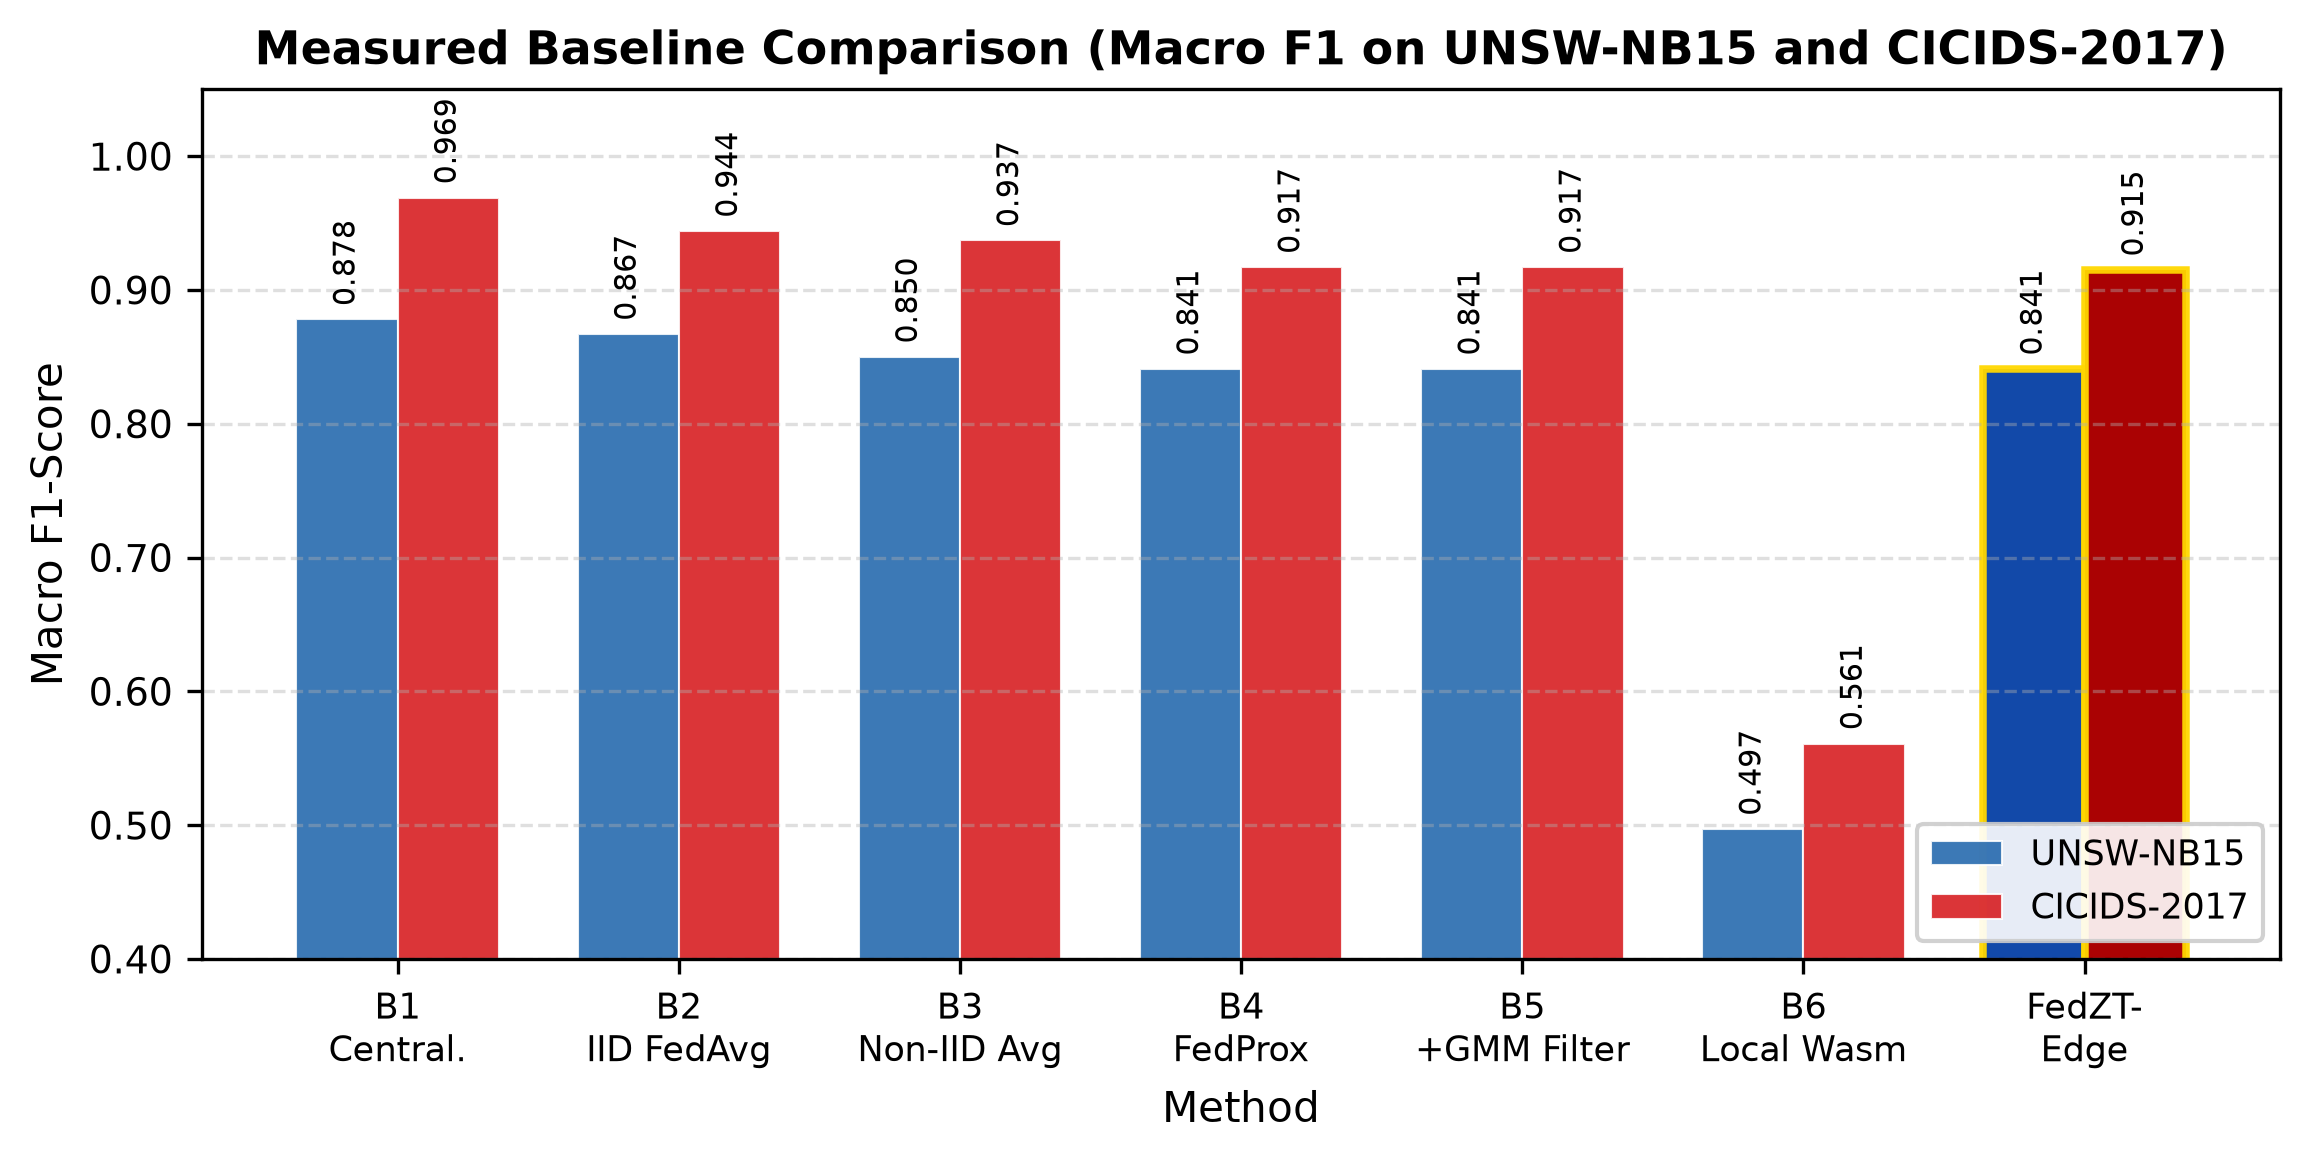
\includegraphics[width=0.88\columnwidth]{fig4_baseline_bar}
\caption{Macro-F1 of all baselines and FedZT-Edge on UNSW-NB15 (blue) and
CICIDS-2017 (red). The isolated baseline B6 is far below the rest, and
FedZT-Edge matches FedProx (B4) on both datasets.}
\label{fig:baseline_bar}
\end{figure}

\subsection{Statistical Significance}

Table~\ref{tab:stats} lists pairwise Welch $t$-tests (Wilcoxon where applicable)
with Holm--Bonferroni correction.

\begin{table}[t]
\centering
\footnotesize
\caption{Pairwise tests of FedZT-Edge against each baseline (Holm-corrected
$p$). $d$: Cohen's $d$. $^{*}$Significant at 0.05.}
\label{tab:stats}
\setlength{\tabcolsep}{3pt}
\begin{tabularx}{\columnwidth}{@{}l c C C c@{}}
\toprule
\textbf{Comparison} & \textbf{Dataset} & \textbf{Holm $p$} & \textbf{$d$} & \textbf{Sig.} \\
\midrule
vs B1 & UNSW   & 0.174 & $-2.87$  & No \\
vs B2 & UNSW   & 0.411 & $-2.35$  & No \\
vs B3 & UNSW   & 1.000 & $-0.43$  & No \\
vs B4 & UNSW   & 1.000 & $+0.00$  & No \\
vs B5 & UNSW   & 1.000 & $+0.00$  & No \\
vs B6 & UNSW   & 0.174 & $+4.46$  & No \\
\midrule
vs B1 & CICIDS & 0.003 & $-10.27$ & Yes$^{*}$ \\
vs B2 & CICIDS & 0.029 & $-5.82$  & Yes$^{*}$ \\
vs B3 & CICIDS & 0.253 & $-2.13$  & No \\
vs B4 & CICIDS & 0.800 & $-0.20$  & No \\
vs B5 & CICIDS & 0.800 & $-0.20$  & No \\
vs B6 & CICIDS & 0.034 & $+8.47$  & Yes$^{*}$ \\
\bottomrule
\end{tabularx}
\end{table}

No UNSW-NB15 comparison survives correction (smallest Holm $p=0.174$). With
three seeds, the tests cannot resolve differences this small. The CICIDS-2017
results are clearer. FedZT-Edge is significantly below B1 (Holm $p=0.003$,
$d=-10.27$) and B2 ($p=0.029$, $d=-5.82$) and significantly above B6
($p=0.034$, $d=+8.47$). The difference to B4 is negligible on both datasets, so
adding zero-trust and Wasm to FedProx costs no detectable accuracy.

\subsection{Adversarial Robustness}

Figure~\ref{fig:adversarial} and Table~\ref{tab:adversarial} show how the
methods degrade as the share of malicious clients grows from 0 to 30\%.

\begin{figure}[!t]
\centering
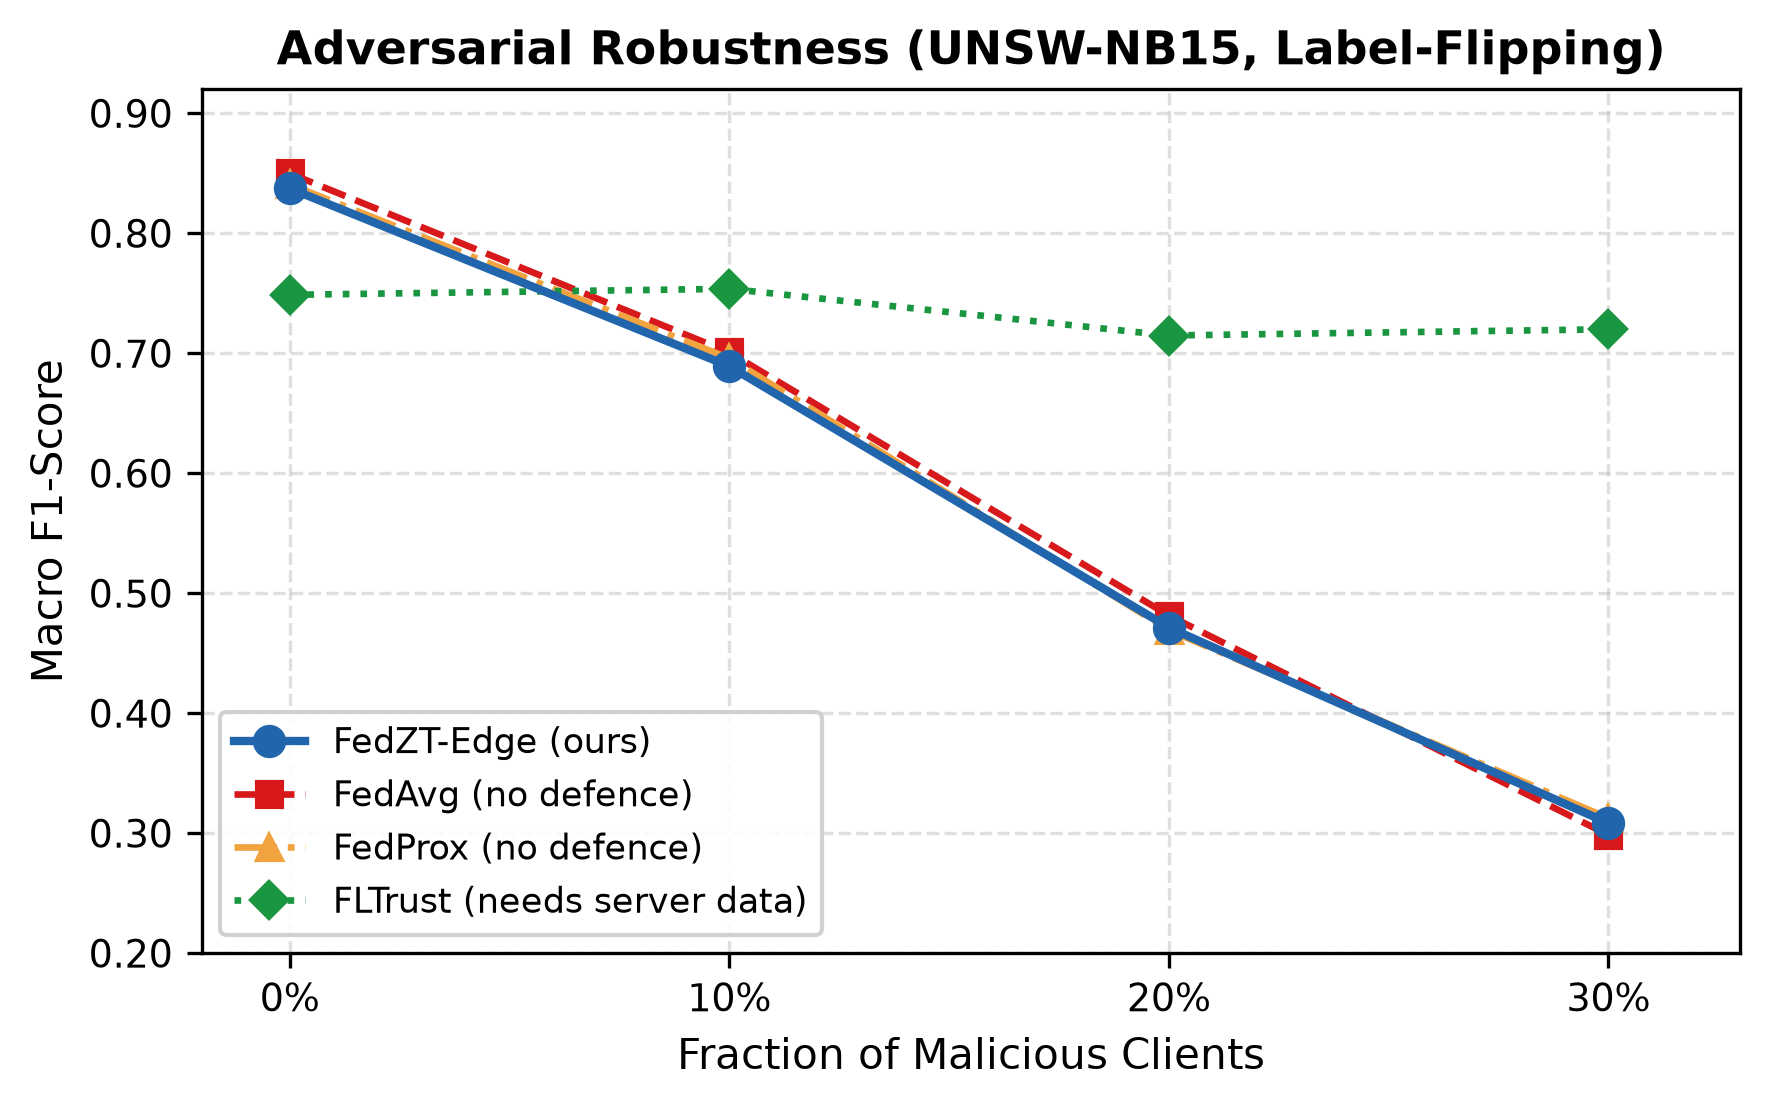
\includegraphics[width=0.88\columnwidth]{fig1_adversarial}
\caption{Macro-F1 against malicious-client rate on UNSW-NB15. FLTrust stays near
0.72, while FedZT-Edge, FedProx and FedAvg all fall sharply beyond 10\%. The
GMM filter helps little on UNSW-NB15 and more on CICIDS-2017.}
\label{fig:adversarial}
\end{figure}

\begin{table*}[t]
\centering
\footnotesize
\caption{Adversarial robustness on UNSW-NB15: macro-F1 (mean$\pm$std, 3 seeds).
FLTrust uses a 100-sample server anchor set.}
\label{tab:adversarial}
\setlength{\tabcolsep}{2.8pt}
\begin{tabularx}{\textwidth}{@{}l CCCC@{}}
\toprule
\textbf{Method} & \textbf{0\%} & \textbf{10\%} & \textbf{20\%} & \textbf{30\%} \\
\midrule
FedAvg (no defence) & $0.850\pm0.021$ & $0.701\pm0.100$ & $0.481\pm0.241$ & $0.299\pm0.377$ \\
FedProx (no filter) & $0.841\pm0.020$ & $0.696\pm0.068$ & $0.469\pm0.193$ & $0.313\pm0.372$ \\
FLTrust (anchor)    & $0.749\pm0.022$ & $0.754\pm0.015$ & $0.715\pm0.028$ & $0.720\pm0.033$ \\
\textbf{FedZT-Edge} & $0.837\pm0.017$ & $0.689\pm0.051$ & $0.471\pm0.180$ & $0.308\pm0.363$ \\
\bottomrule
\end{tabularx}

\smallskip
\par\raggedright\footnotesize
FLTrust is far ahead of FedZT-Edge at high attack rates (F1 of 0.720 against
0.308 at 30\%) but needs labelled data on the server, which the privacy model of
FedZT-Edge rules out. On CICIDS-2017, a separately reported 30\% attack result
gives F1\,=\,0.909, against 0.845 for FedAvg and 0.836 for FedProx. This does
not reconcile with the 20\% attack filter ablation (F1\,=\,0.831), and the run
configurations are not available, so the figures should not be read as one
trend. The 0\% value of 0.837 comes from the adversarial-evaluation runs and
differs by 0.003 from the baseline run (0.841), which is within seed-to-seed
variation.
\end{table*}

On UNSW-NB15 the filter has precision 1.0 at every attack rate, but recall drops
to 0 at 20 to 30\%. Label flipping does not inflate update norms (maximum norm
ratio 1.09 against a limit of 4), so Stage~A never fires. Under the actual
Dirichlet $\alpha=0.5$ experiment, Stage~B also did not fire at any attack rate
in any of the three seeds. The filter therefore has zero recall at 20 to 30\%
attack, and a precision of 1.0 carries no information when no malicious update
is flagged. An earlier IID diagnostic does not represent these conditions. On
CICIDS-2017 the filter's recall is 0.667 at 10\% attack and 0.500 at 20\%, which
explains the stronger protection there.

\begin{table}[t]
\centering
\footnotesize
\caption{Reported update-filter diagnostics. NR = not reported in the experiment record.}
\label{tab:filter-diagnostics}
\begin{tabularx}{\columnwidth}{@{}Y c c c@{}}
\toprule
Dataset / attack & Precision & Recall & Stage B\\fires?\\
\midrule
UNSW-NB15, 10\% & 1.000 & NR & No\\
UNSW-NB15, 20\% & 1.000 & 0.000 & No\\
UNSW-NB15, 30\% & 1.000 & 0.000 & No\\
CICIDS-2017, 10\% & NR & 0.667 & NR\\
CICIDS-2017, 20\% & NR & 0.500 & NR\\
\bottomrule
\end{tabularx}
\end{table}

\subsection{Convergence Behaviour}

Figure~\ref{fig:convergence} plots macro-F1 per global round for FedZT-Edge and
three baselines at $\alpha=0.5$.

\begin{figure}[!t]
\centering
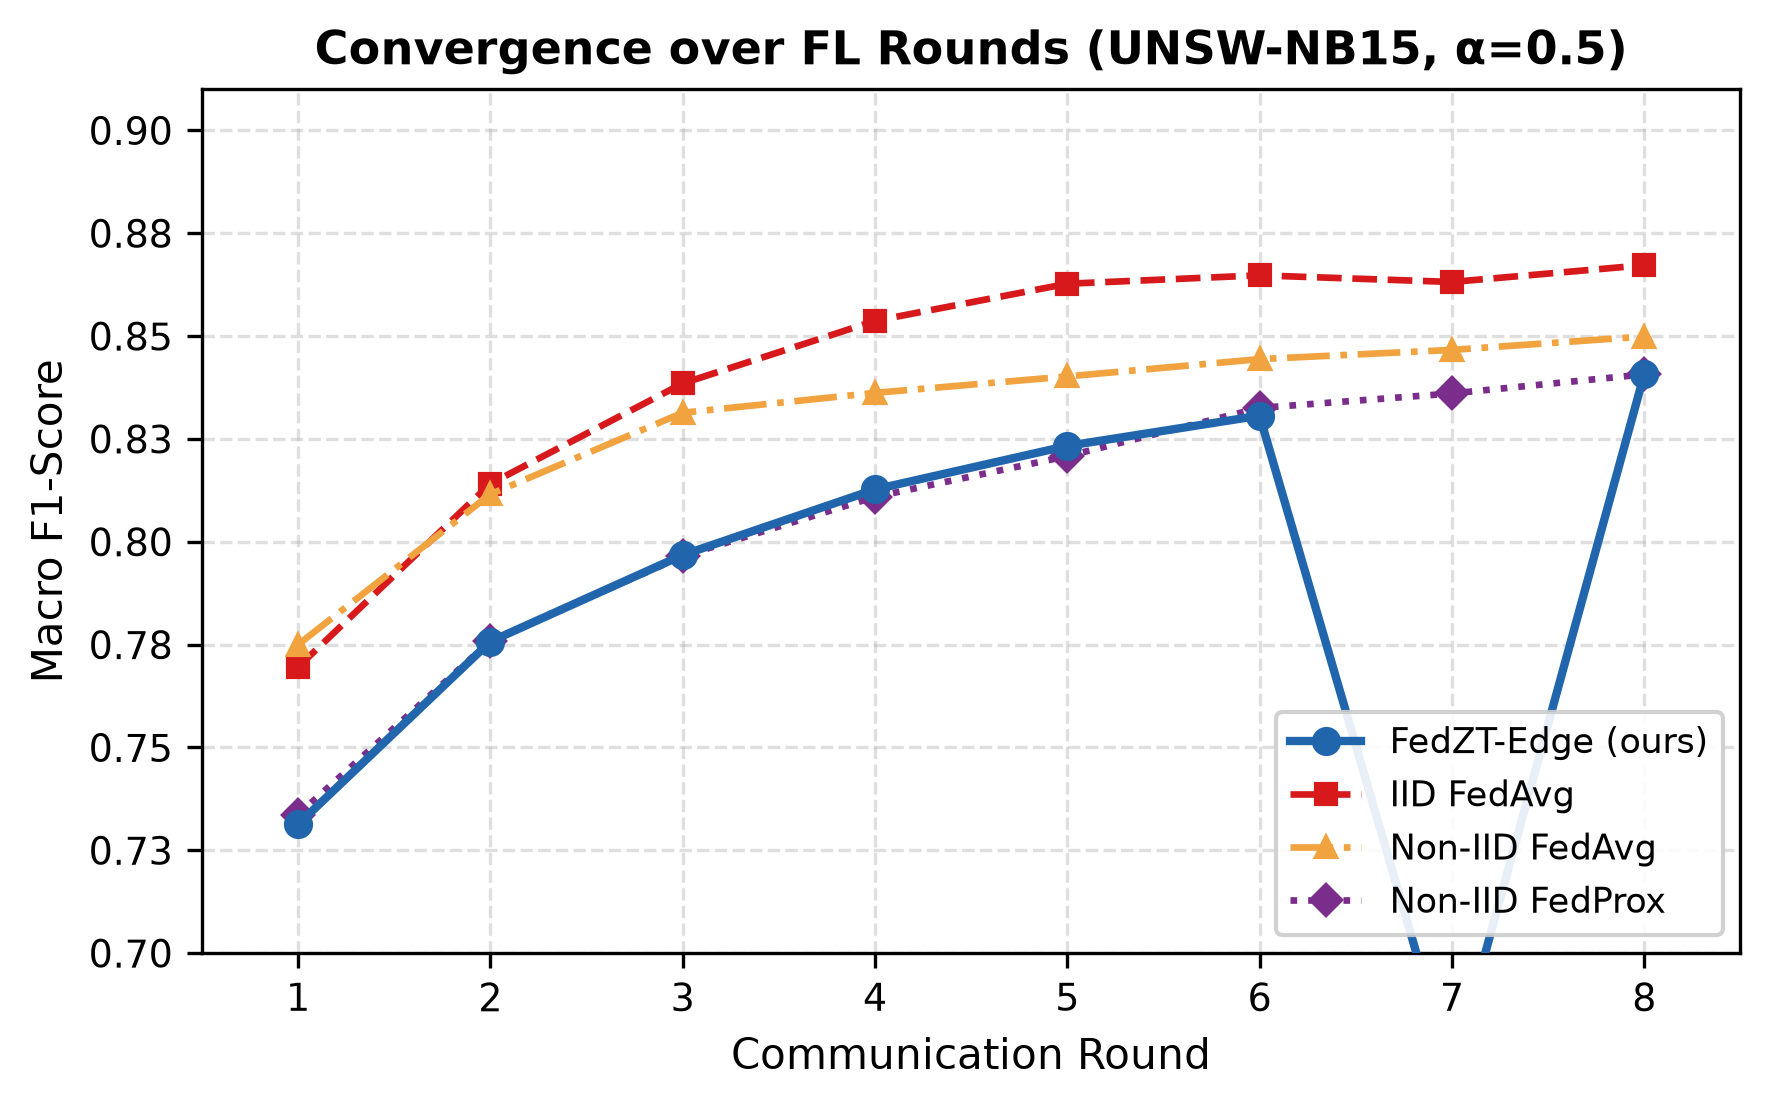
\includegraphics[width=0.88\columnwidth]{fig3_convergence}
\caption{Macro-F1 per global round on UNSW-NB15 at $\alpha=0.5$ for FedZT-Edge,
IID FedAvg, non-IID FedAvg and non-IID FedProx.}
\label{fig:convergence}
\end{figure}

The trace covers UNSW-NB15 only. The curve dips near round 7, so it is neither
smooth nor monotonic. FedAvg, which has no proximal term, varies more across
seeds, especially on UNSW-NB15 where class imbalance is stronger.

\subsection{Heterogeneity Sensitivity}

Figure~\ref{fig:heterogeneity} shows macro-F1 over four Dirichlet $\alpha$
values for FedZT-Edge, FedAvg, FedProx and FedNova.

\begin{figure}[!t]
\centering
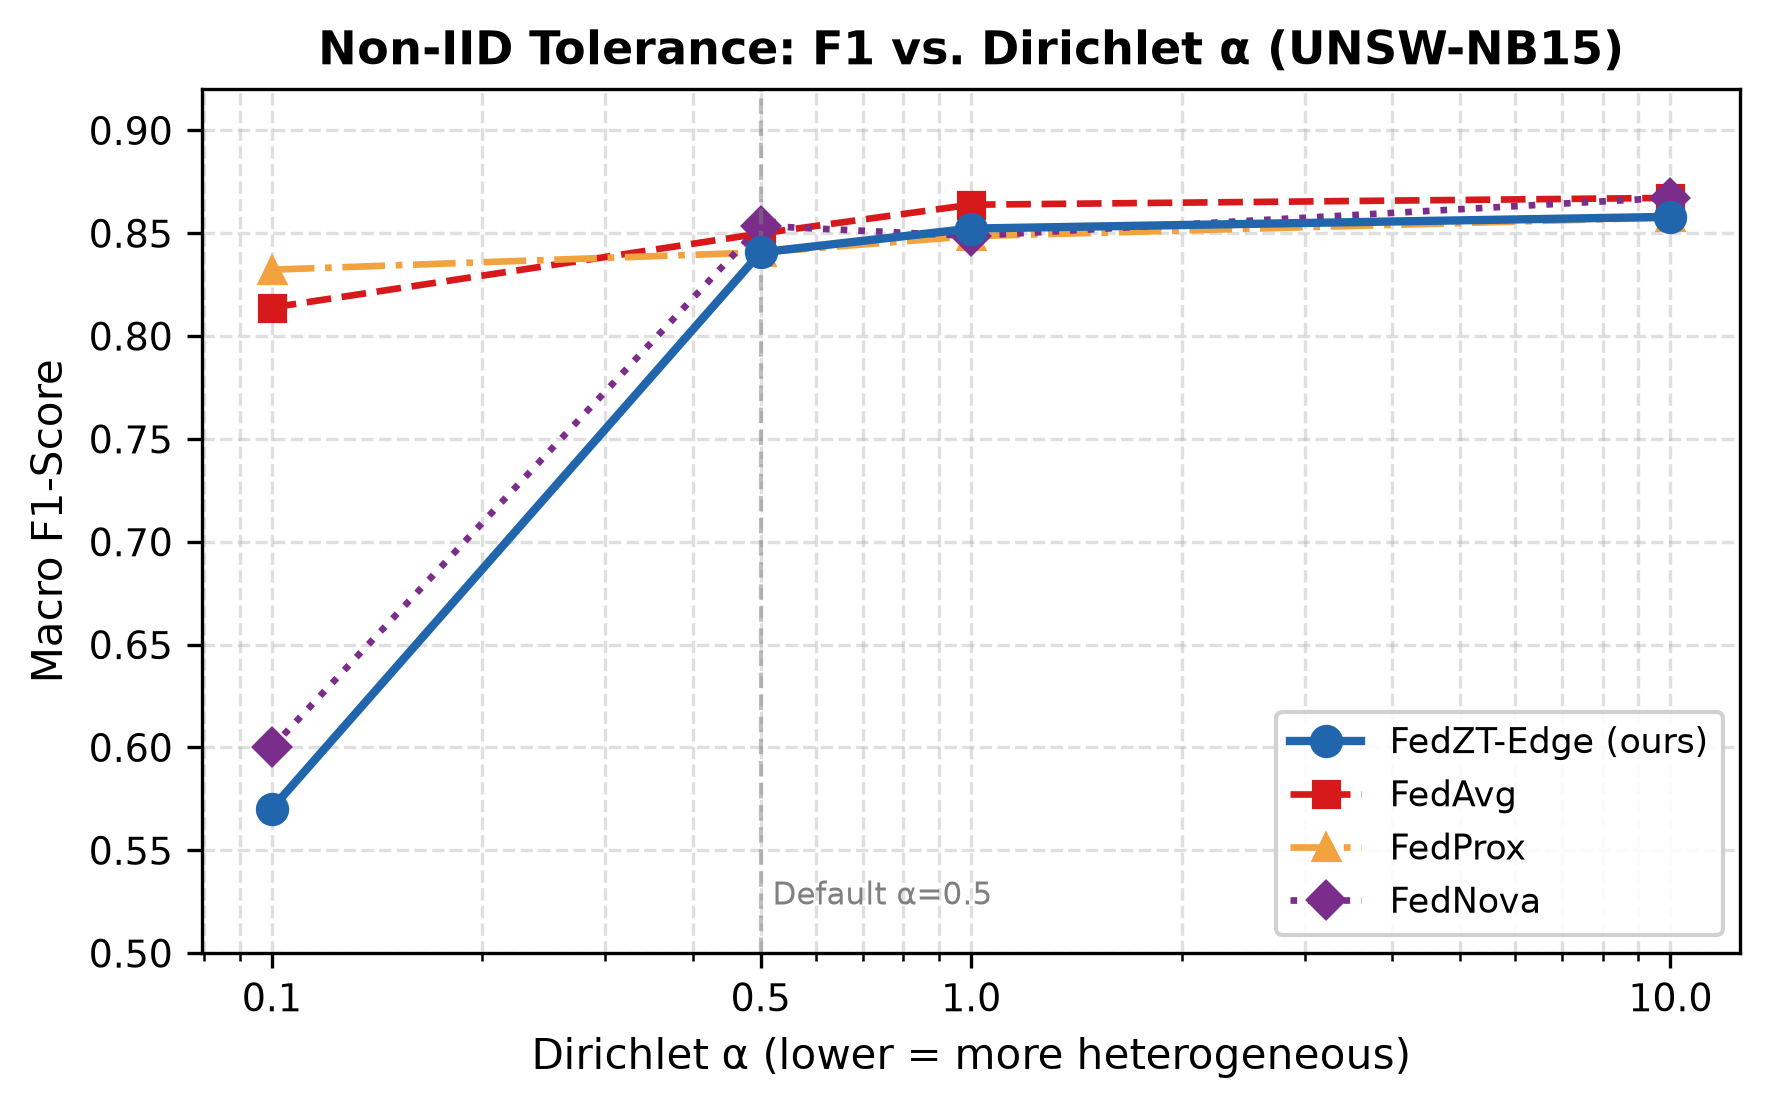
\includegraphics[width=0.88\columnwidth]{fig2_heterogeneity}
\caption{Macro-F1 against Dirichlet $\alpha$ on UNSW-NB15. All methods improve
as the data become more IID. At $\alpha=0.1$ FedZT-Edge is 26\,pp below
FedProx.}
\label{fig:heterogeneity}
\end{figure}

For $\alpha\ge0.5$ FedZT-Edge tracks FedProx closely in the reported runs. At
$\alpha=0.1$ on UNSW-NB15 it falls to F1\,=\,0.570 while FedProx reaches 0.832.
CICIDS-2017 shows the same pattern: 0.767 for FedZT-Edge and 0.915 for FedNova.
The likely explanation is that extreme skew makes honest updates look like
outliers to the GMM filter, so legitimate contributions are rejected. This was
not tested directly.

\subsection{System Overhead}

Figure~\ref{fig:energy} shows the analytical resource model for three hardware
tiers, and Table~\ref{tab:ablation} holds the latencies measured on the laptop.

\begin{figure}[!t]
\centering
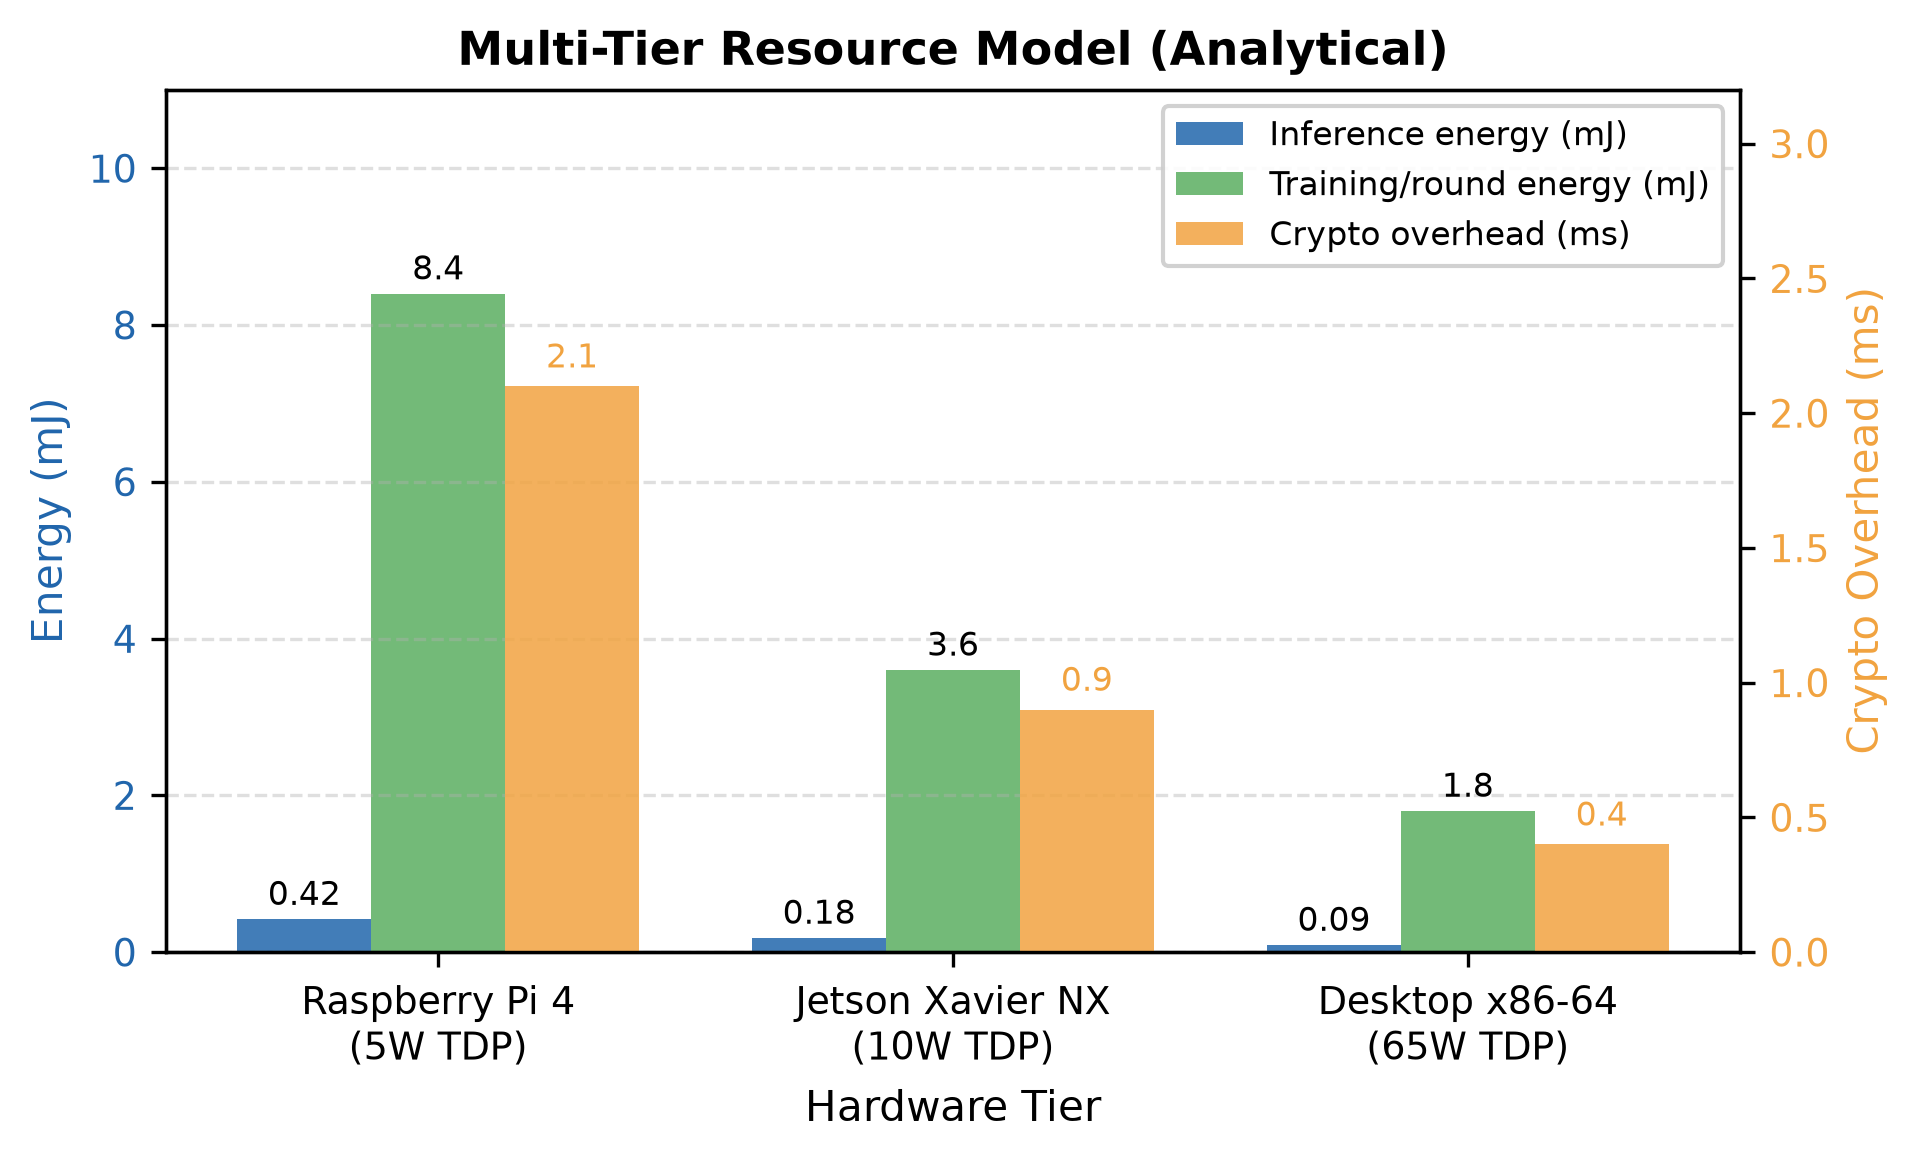
\includegraphics[width=0.88\columnwidth]{fig5_energy}
\caption{Analytical energy and cryptographic-overhead model across three
hardware tiers (Raspberry Pi~4, Jetson Xavier NX, desktop x86-64). The values
are derived from profiled CPU cycles, not from physical measurement.}
\label{fig:energy}
\end{figure}

Enabling AES-256-GCM and RSA-2048 adds 0.616\,ms per round on UNSW-NB15 (1.785
against 1.169\,ms) and 0.600\,ms on CICIDS-2017. Wasm batch latency is 0.375\,ms
on UNSW-NB15 and 0.276\,ms on CICIDS-2017, against native latencies of 0.300 and
0.177\,ms, an overhead of 25\% and 56\%. Memory rises from 1.21\,MB (native) to
4.21\,MB (Wasm), well inside the 8\,MB or more of DRAM on most edge SoCs.

\section{Comparison with Base Papers and Prior Work}\label{sec:comparison}

\subsection{Summary of Base Papers}

Table~\ref{tab:basepaper_summary} lists the studies whose problem statements,
methods or datasets shaped FedZT-Edge, with the limitation of each.

\begin{table*}[t]
\centering
\scriptsize
\caption{Base papers. F1: macro-F1; Acc: accuracy; FL: federated learning.}
\label{tab:basepaper_summary}
\setlength{\tabcolsep}{3pt}
\begin{tabularx}{\textwidth}{@{}P{2.6cm} Y Y Y P{1.6cm} Y Y@{}}
\toprule
\textbf{Authors (year)} & \textbf{Problem} & \textbf{Method} & \textbf{Dataset} &
\textbf{Metric} & \textbf{Result} & \makecell{\textbf{Key}\\\textbf{limitation}} \\
\midrule
McMahan et al.\ (2017)~\cite{mcmahan2017} & Private distributed training & FedAvg & MNIST, Shakespeare & Accuracy & High on IID data & Collapses under non-IID data \\
Li et al.\ (2020)~\cite{li2020federated} & Non-IID convergence & FedProx & MNIST, FEMNIST, Shakespeare & Accuracy & Better non-IID convergence & No security layer \\
Tolpegin et al.\ (2020)~\cite{tolpegin2020} & Label-flipping attacks on FL & Attack analysis with cosine-distance detection & MNIST, KDD99 & F1, attack success rate & F1 collapses beyond 30\% attack & Detection only, no full defence \\
Cao et al.\ (2021)~\cite{cao2021fltrust} & Byzantine-robust aggregation & FLTrust (server-anchor trust scores) & MNIST, CIFAR-10 & F1, accuracy & F1\,=\,0.72 at 30\% malicious & Needs labelled server data \\
Moustafa \& Slay (2015)~\cite{moustafa2015unsw} & Intrusion-detection benchmark & Traffic capture and labelling & UNSW-NB15 & Accuracy, F1 & Standard benchmark & Centralised \\
Mahida (2022)~\cite{mahida2022} & Centralised IDS & Chi-square + MLP & UNSW-NB15 & Accuracy & Acc\,$>$\,95\% & Centralised, one dataset \\
Albogami et al.\ (2023)~\cite{albogami2023} & Deep-learning IDS & Multi-layer DNN & CICIDS-2017 & F1, accuracy & F1\,$>$\,0.96, Acc\,$>$\,0.97 & Centralised, no adversarial test \\
\midrule
\textbf{FedZT-Edge (this work)} & Federated zero-trust Wasm IDS & FedProx + GMM filter + DRL + Wasm & UNSW-NB15, CICIDS-2017 & F1, accuracy & F1\,=\,0.841 / 0.915 & DQN undertrained; no physical edge hardware \\
\bottomrule
\end{tabularx}
\end{table*}

\subsection{Quantitative Comparison}

Table~\ref{tab:comparison} compares FedZT-Edge numerically with each base
method. All FedZT-Edge numbers use 10 clients, $\alpha=0.5$, 8 rounds and seeds
$[42,101,2024]$. Entries marked $(\dagger)$ were re-implemented in this setting;
entries marked $(\star)$ are copied from the original papers and may come from
different configurations.

\begin{table*}[t]
\centering
\scriptsize
\caption{Comparison of FedZT-Edge with base papers. $(\dagger)$: re-implemented
here. $(\star)$: taken from the original paper. ``---'': not reported.
$\Delta$F1 is F1 of FedZT-Edge minus F1 of the listed method. The FLTrust
$\Delta$F1 uses the 0.837 clean-setting value from Table~\ref{tab:adversarial}.}
\label{tab:comparison}
\setlength{\tabcolsep}{2.8pt}
\begin{tabularx}{\textwidth}{@{}P{3.6cm} CCC CCC c@{}}
\toprule
\multirow{2}{*}{\textbf{Method}} &
\multicolumn{3}{c}{\textbf{UNSW-NB15}} & \multicolumn{3}{c}{\textbf{CICIDS-2017}} &
\multirow{2}{*}{\textbf{Source}} \\
\cmidrule(lr){2-4}\cmidrule(lr){5-7}
& \textbf{F1} & \textbf{Acc} & \textbf{$\Delta$F1} &
  \textbf{F1} & \textbf{Acc} & \textbf{$\Delta$F1} & \\
\midrule
Centralised MLP (B1)           & 0.878 & 0.864 & $-0.037$ & 0.969 & 0.979 & $-0.054$ & $(\dagger)$ \\
IID FedAvg (B2)                & 0.867 & 0.851 & $-0.026$ & 0.944 & 0.963 & $-0.029$ & $(\dagger)$ \\
Non-IID FedAvg (B3)            & 0.850 & 0.830 & $-0.009$ & 0.937 & 0.959 & $-0.022$ & $(\dagger)$ \\
FedProx $\mu=0.1$ (B4)         & 0.841 & 0.819 & $\pm0.000$ & 0.917 & 0.947 & $-0.002$ & $(\dagger)$ \\
Local Wasm-only (B6)           & 0.497 & 0.612 & $+0.344$ & 0.561 & 0.688 & $+0.354$ & $(\dagger)$ \\
FLTrust~\cite{cao2021fltrust} (0\% attack) & 0.749 & --- & $+0.088$ & --- & --- & --- & $(\dagger)$ \\
Mahida~\cite{mahida2022}       & --- & $>$0.95 & --- & --- & --- & --- & $(\star)$ \\
Albogami~\cite{albogami2023}   & --- & --- & --- & $>$0.960 & $>$0.970 & $<-0.045$ & $(\star)$ \\
\midrule
\textbf{FedZT-Edge (the proposed method)}     & \textbf{0.841} & \textbf{0.823} & --- & \textbf{0.915} & \textbf{0.946} & --- & $(\dagger)$ \\
\bottomrule
\end{tabularx}
\end{table*}

\subsection{Methodological Comparison}

Table~\ref{tab:method_diff} contrasts the design of FedZT-Edge with the methods
it builds on.

\begin{table*}[t]
\centering
\small
\caption{Design comparison of FedZT-Edge with FedAvg, FedProx and FLTrust.}
\label{tab:method_diff}
\setlength{\tabcolsep}{3pt}
\begin{tabularx}{\textwidth}{@{}P{2.5cm} Y Y Y Y@{}}
\toprule
\textbf{Feature} & \textbf{FedZT-Edge} & \textbf{FedAvg} & \textbf{FedProx} & \textbf{FLTrust} \\
\midrule
Aggregation       & FedProx        & FedAvg & FedProx  & Trust-weighted \\
Poisoning defence & GMM filter & None   & None     & Server anchor \\
Trust enforcement & DRL (DQN)      & None   & None     & Score threshold \\
Inference sandbox & Wasm           & None   & None     & None \\
Server data       & No             & No     & No       & Yes \\
Non-IID handling  & Proximal term  & None   & Proximal & Partial \\
\bottomrule
\end{tabularx}
\end{table*}

FedAvg~\cite{mcmahan2017} averages client updates with no mechanism for
divergent ones. FedZT-Edge replaces it with FedProx, filters outlier updates
before aggregation and adds a DRL trust layer. FedProx~\cite{li2020federated} is
used directly for aggregation, and FedZT-Edge matches its F1 on UNSW-NB15
(0.841) and nearly matches it on CICIDS-2017 (0.915 against 0.917), so the
security layers are close to accuracy-neutral. Tolpegin et
al.~\cite{tolpegin2020} identified the label-flipping weakness but built no
system-level defence. FedZT-Edge adds the filter of Algorithm~\ref{alg:filter},
based on update norms and pairwise cosine distances, and connects it to
zero-trust enforcement.

FLTrust~\cite{cao2021fltrust} is much more robust at high attack rates (F1 of
0.720 at 30\% malicious clients against 0.308 for FedZT-Edge on UNSW-NB15), but
it keeps a clean labelled dataset on the server. That conflicts with the privacy
contract of FedZT-Edge, where the server holds no labelled data, so the design
accepts lower robustness in exchange for stronger privacy. Mahida~\cite{mahida2022}
and Albogami et al.~\cite{albogami2023} train centralised models on pooled data
and reach Acc\,$>$\,95\% and F1\,$>$\,0.96. The 1,234-parameter MLP of
FedZT-Edge sees only local 20-feature data, while Albogami et al.\ use a far
larger DNN on the full dataset. Their numbers therefore mark a ceiling and are
not a like-for-like benchmark.

\subsection{Improvement Analysis}

Table~\ref{tab:improvement} gives the absolute and relative F1 change of
FedZT-Edge against each base method.

\begin{table*}[t]
\centering
\small
\caption{Absolute ($\Delta$F1) and relative ($\Delta$F1\%) change of FedZT-Edge
against each base method. Positive means FedZT-Edge is better. Relative change
is $\Delta\text{F1}/\text{F1}_{\text{base}}\times100$.}
\label{tab:improvement}
\setlength{\tabcolsep}{3pt}
\begin{tabularx}{\textwidth}{@{}P{3.0cm} CCCC@{}}
\toprule
\multirow{2}{*}{\textbf{Base method}} &
\multicolumn{2}{c}{\textbf{UNSW-NB15}} & \multicolumn{2}{c}{\textbf{CICIDS-2017}} \\
\cmidrule(lr){2-3}\cmidrule(lr){4-5}
& $\Delta$\textbf{F1} & $\Delta$\textbf{F1\%} & $\Delta$\textbf{F1} & $\Delta$\textbf{F1\%} \\
\midrule
B1 (centralised)    & $-0.037$   & $-4.2\%$  & $-0.054$ & $-5.6\%$ \\
B2 (IID FedAvg)     & $-0.026$   & $-3.0\%$  & $-0.029$ & $-3.1\%$ \\
B3 (non-IID FedAvg) & $-0.009$   & $-1.1\%$  & $-0.022$ & $-2.3\%$ \\
B4 (FedProx)        & $\pm0.000$ & $0.0\%$   & $-0.002$ & $-0.2\%$ \\
B6 (local only)     & $+0.344$   & $+69.2\%$ & $+0.354$ & $+63.1\%$ \\
FLTrust (0\%)       & $+0.088$   & $+11.7\%$ & ---      & --- \\
Albogami (DNN)      & ---        & ---       & $<-0.045$ & $<-4.7\%$ \\
\bottomrule
\end{tabularx}
\end{table*}

The largest gain is over the isolated baseline B6, a relative improvement of
69.2\% on UNSW-NB15 and 63.1\% on CICIDS-2017. Federated training clearly beats
training alone, even with the filter, encryption and Wasm runtime in place.

FedProx (B4) is the most relevant comparison because it works under the same
privacy model. FedZT-Edge matches it on UNSW-NB15 and is 0.002 lower on
CICIDS-2017, a difference that is not statistically distinguishable (Holm
$p=0.80$, $d=-0.20$). On these data the security stack costs no measurable
accuracy. The lower scores against B1 to B3 cannot be attributed to filter
rejection at $\alpha=0.5$, because B4 and B5 are identical and the filter flags
no updates. The individual contributions of the privacy-preserving split and the
proximal optimisation were not isolated.

At zero attack FedZT-Edge scores 11.7\% higher F1 than FLTrust (0.837 against
0.749). One possible reason is that the trust weighting of FLTrust, tuned for
adversarial conditions, down-weights some honest clients even when nobody
attacks. This was not investigated.

\subsection{Limits of the Comparison}

McMahan et al., Li et al.\ and Cao et al.\ evaluate on image or text benchmarks,
not on UNSW-NB15 or CICIDS-2017. The re-implemented baselines (B1 to B6 and
FLTrust) share the train/test partition and Dirichlet split with FedZT-Edge, so
those comparisons are fair. Mahida and Albogami use their own splits and
preprocessing, so a direct F1 comparison is not appropriate; Table~\ref{tab:comparison}
marks their numbers with $(\star)$. Albogami et al.\ also use a much larger DNN,
and larger models usually score higher on centralised IDS tasks. The model here
is small on purpose, to fit edge memory budgets. All baselines ran on the same
laptop, so runtime and energy cannot be compared with numbers from other papers.
FLTrust clearly beats FedZT-Edge at 30\% malicious clients (Table~\ref{tab:adversarial}),
but its server anchor dataset is a weaker privacy assumption than FedZT-Edge
allows. Finally, the DQN was not trained to convergence, so the DQN rows in
Table~\ref{tab:ablation} say little about a mature RL policy.

\section{Ablation Study}\label{sec:ablation}

Table~\ref{tab:ablation} varies eight design choices one at a time while holding
the rest fixed. The unit depends on the axis: F1 for detection, mean cumulative
reward for the DRL axis, latency in milliseconds for the runtime axes, and
action alignment in percent for the partition test.

\begin{table*}[t]
\centering
\scriptsize
\caption{Ablation results over eight axes (seeds $[42,101,2024]$). F1: macro-F1
(mean and std); Reward: mean cumulative DRL reward; Latency: batch latency (ms);
Align.: action alignment (\%) under network partition. $^{\dagger}$DQN not
trained to convergence.}
\label{tab:ablation}
\setlength{\tabcolsep}{2.8pt}
\begin{tabularx}{\textwidth}{@{}c P{3.8cm} P{3.2cm} CC CC@{}}
\toprule
\textbf{ID} & \textbf{Design axis} & \textbf{Variant} &
\multicolumn{2}{c}{\textbf{UNSW-NB15}} & \multicolumn{2}{c}{\textbf{CICIDS-2017}} \\
\cmidrule(lr){4-5}\cmidrule(lr){6-7}
& & & \textbf{Value} & \textbf{Std} & \textbf{Value} & \textbf{Std} \\
\midrule
\multirow{2}{*}{(a)} & \multirow{2}{*}{Update filter (20\% attack)}
  & Disabled & 0.462 & 0.180 & 0.807 & 0.111 \\
& & Enabled  & 0.471 & 0.180 & 0.831 & 0.123 \\
\cmidrule(lr){1-7}
\multirow{4}{*}{(b)} & \multirow{4}{*}{FedProx $\mu$ at $\alpha=0.1$}
  & $\mu=0.01$ & 0.756 & 0.078 & 0.902 & 0.029 \\
& & $\mu=0.1$  & 0.832 & 0.037 & 0.891 & 0.017 \\
& & $\mu=0.5$  & 0.778 & 0.012 & 0.876 & 0.018 \\
& & $\mu=1.0$  & 0.750 & 0.002 & 0.793 & 0.032 \\
\cmidrule(lr){1-7}
\multirow{3}{*}{(c)} & \multirow{3}{*}{Feature count $k$}
  & $k=10$ & 0.794 & 0.005 & 0.890 & 0.006 \\
& & $k=20$ & 0.837 & 0.017 & 0.915 & 0.005 \\
& & $k=30$ & 0.894 & 0.003 & 0.918 & 0.001 \\
\cmidrule(lr){1-7}
\multirow{2}{*}{(d)$^{\dagger}$} & \multirow{2}{*}{Mitigation engine (reward)}
  & DQN adaptive     & $-1.137$ & 3.100 & $-0.195$ & 2.965 \\
& & Static threshold & $+2.049$ & 0.825 & $+2.024$ & 0.743 \\
\cmidrule(lr){1-7}
\multirow{2}{*}{(e)} & \multirow{2}{*}{Crypto envelope (latency, ms)}
  & Disabled (plaintext) & 1.169 & 0.030 & 0.925 & 0.107 \\
& & Enabled (AES+RSA)    & 1.785 & 0.145 & 1.525 & 0.227 \\
\cmidrule(lr){1-7}
\multirow{2}{*}{(f)} & \multirow{2}{*}{Runtime (latency, ms)}
  & Native & 0.300 & 0.027 & 0.177 & 0.037 \\
& & Wasm   & 0.375 & 0.058 & 0.276 & 0.070 \\
\cmidrule(lr){1-7}
\multirow{2}{*}{(g)} & \multirow{2}{*}{Network churn (F1)}
  & 0\% dropout  & 0.837 & 0.017 & 0.915 & 0.005 \\
& & 20\% dropout & 0.692 & 0.207 & 0.909 & 0.019 \\
\cmidrule(lr){1-7}
\multirow{2}{*}{(h)} & \multirow{2}{*}{ZT availability (align., \%)}
  & PDP online (normal)        & 100.0 & 0.0 & 100.0 & 0.0 \\
& & Local fallback (partition) & 49.0  & 1.5 & 64.8  & 1.5 \\
\bottomrule
\end{tabularx}
\end{table*}

\textbf{(a) Update filter.} At 20\% attack the filter raises F1 by 0.009 on
UNSW-NB15 and 0.024 on CICIDS-2017. The UNSW-NB15 gain is smaller than the
seed-to-seed spread, so three runs cannot confirm it. The CICIDS-2017 gain is
more consistent, which suggests the filter helps more when local traffic
distributions are easier to separate.

\textbf{(b) Proximal term $\mu$.} At $\alpha=0.1$, $\mu=0.1$ gives the best F1 on
UNSW-NB15, by modest margins. On CICIDS-2017, $\mu=0.01$ beats $\mu=0.1$ by
1.1\,pp, so the best value depends on the dataset. A large $\mu$ hurts both,
probably because it over-constrains local training.

\textbf{(c) Feature count.} F1 rises with $k$ on both datasets. The $k=20$
setting is kept for consistency with the main experiments, although UNSW-NB15 F1
is 0.057 higher at $k=30$. No on-device feature-selection cost was measured, so
the evidence does not establish an efficiency advantage for $k=20$.

\textbf{(d) DRL policy engine.} The undertrained DQN earns a negative mean reward
($-1.14$ on UNSW-NB15, $-0.19$ on CICIDS-2017), while the hand-tuned static
threshold earns $+2.05$ and $+2.02$. This is the weakest part of the system. The
results do not establish DQN effectiveness, and a converged, controlled
evaluation is required.

\textbf{(e) Cryptographic envelope.} AES-256-GCM with RSA-2048 adds 0.616\,ms on
UNSW-NB15 and 0.600\,ms on CICIDS-2017. Edge uplinks typically add 10 to
100\,ms of network latency, so this cost is small in practice.

\textbf{(f) Wasm runtime.} Wasm is 25\% slower than native on UNSW-NB15 (0.375
against 0.300\,ms) and 56\% slower on CICIDS-2017 (0.276 against 0.177\,ms).
Both stay under 1\,ms per batch, and memory grows from 1.21 to 4.21\,MB.

\textbf{(g) Network churn.} With 20\% dropout, UNSW-NB15 F1 falls by 14.5\,pp
with large variance across seeds, while CICIDS-2017 F1 falls by only 0.6\,pp.
UNSW-NB15 is more imbalanced, so losing a client that holds many minority-class
samples may hurt the global model more. This explanation was not tested.

\textbf{(h) Zero-trust availability under partition.} When the PDP is
unreachable, the cached snapshot agrees with the full policy on 49\% of actions
for UNSW-NB15 and 64.8\% for CICIDS-2017. With four actions, random choice would
agree 25\% of the time, so the UNSW-NB15 snapshot is only moderately useful and
the CICIDS-2017 snapshot is more reliable.

\section{Discussion}\label{sec:discussion}

\subsection{Where the System Works and Where It Does Not}

FedZT-Edge behaves well at moderate heterogeneity ($\alpha\ge0.5$). The proximal
term keeps local models from drifting far, so cosine distances between client
updates stay small and the filter lets most updates through. The encryption layer
and the Wasm sandbox do not alter gradient values and cannot affect model
quality.

At $\alpha=0.1$ the behaviour changes. On UNSW-NB15 the gap to FedProx grows to
26.2\,pp. A likely cause is that very skewed local data produce updates far from
the global mean even when every client is honest. The filter then flags honest
updates, and the DRL agent may down-weight or quarantine well-behaved clients,
which adds to the loss.

Under heavy poisoning ($\ge20\%$ malicious clients on UNSW-NB15) the filter's
recall falls to zero, so malicious updates reach aggregation. Label-flipped
updates keep honest-like norms, so Stage~A does not fire, and Stage~B did not
fire in any seed or attack-rate condition at $\alpha=0.5$. This is the regime
where defence matters most. FLTrust avoids the problem with a clean server
dataset, at the cost of the privacy contract that FedZT-Edge keeps.

\subsection{Research Gaps Addressed}

\textbf{G1}, privacy-preserving edge IDS, is met: no raw sample leaves a client
at any point. \textbf{G2}, non-IID robustness, is partly met: the system holds up
for $\alpha\ge0.5$ but degrades clearly at $\alpha=0.1$. \textbf{G3}, Wasm
deployment feasibility, is also partly met: overhead is within budget on the
laptop, but nothing has been validated on dedicated edge hardware.

\subsection{Threats to Validity}

\textbf{Internal validity.} Three seeds are enough to estimate variance but not
to establish significance on UNSW-NB15, where every Holm-corrected $p$-value
exceeds 0.17. Conclusions for that dataset are exploratory until more seeds are
run.

\textbf{External validity.} Both datasets are lab captures with known class
distributions, whereas real edge traffic keeps changing. The DQN agent is not
ready for production, and the energy model rests on profiled CPU cycles instead
of power measurements.

\textbf{Construct validity.} The ``edge'' here is a laptop running Wasmtime. That
is a reasonable proxy for Wasm runtime overhead but ignores the memory
bandwidth, thermal throttling and real-time scheduling limits of
microcontroller-class hardware.

\section{Conclusion and Future Work}\label{sec:conclusion}

This paper presented FedZT-Edge, a framework that combines federated learning,
zero-trust access control and WebAssembly sandboxing for intrusion detection on
edge networks. Under non-IID partitioning it reaches macro-F1 of 0.841 on
UNSW-NB15 and 0.915 on CICIDS-2017, in line with FedProx, keeps all raw traffic
local, and adds less than a millisecond of cryptographic and runtime overhead.
The proximal term and GMM filter work at moderate heterogeneity but weaken at
$\alpha=0.1$ and under heavy poisoning.

Future work will train the DQN to convergence, measure filter precision and
recall across repeated runs, isolate Stage~A and Stage~B, validate the Wasm
module on physical edge hardware, and evaluate additional robust aggregation
methods and newer IDS datasets.

\section*{Declarations}

\textbf{Data availability.} UNSW-NB15~\cite{moustafa2015unsw} and
CICIDS-2017~\cite{sharafaldin2018cicids} are publicly available from their
project repositories.

\textbf{Code availability.} A public repository URL was not supplied in the
project materials, so public code availability cannot be claimed in this
version.

\textbf{Conflict of interest.} The authors declare no conflict of interest.

\textbf{Funding.} No external funding was received for this study.

\textbf{Use of AI tools.} AI tools were used to generate LaTeX code, to fix the
formatting of tables, and for language editing of the final text. The Antigravity
tool was used to run the experiments. The research design, implementation and
analysis were carried out by the authors, who take full responsibility for the
content and results.

\begingroup\scriptsize
\setlength{\itemsep}{0pt}
\setlength{\parskip}{0pt}
\setlength{\parsep}{0pt}
\begin{thebibliography}{99}

\bibitem{mcmahan2017}
McMahan, H.B., Moore, E., Ramage, D., Hampson, S., Ag{\"u}era y Arcas, B.:
Communication-efficient learning of deep networks from decentralized data.
In: Proceedings of the 20th International Conference on Artificial Intelligence
and Statistics (AISTATS), pp.\ 1273--1282 (2017)

\bibitem{li2020federated}
Li, T., Sahu, A.K., Zaheer, M., Sanjabi, M., Talwalkar, A., Smith, V.:
Federated optimization in heterogeneous networks (FedProx).
In: Proceedings of the 3rd MLSys Conference, pp.\ 429--450 (2020)

\bibitem{tolpegin2020}
Tolpegin, V., Truex, S., Gursoy, M.E., Liu, L.:
Data poisoning attacks against federated learning systems.
In: Proceedings of the European Symposium on Research in Computer Security
(ESORICS), Lecture Notes in Computer Science, vol.\ 12308, pp.\ 480--501 (2020)

\bibitem{bagdasaryan2020}
Bagdasaryan, E., Veit, A., Hua, Y., Estrin, D., Shmatikov, V.:
How to backdoor federated learning.
In: Proceedings of the 23rd International Conference on Artificial Intelligence
and Statistics (AISTATS), pp.\ 2938--2948 (2020)

\bibitem{cao2021fltrust}
Cao, X., Fang, M., Liu, J., Gong, N.Z.:
FLTrust: Byzantine-robust federated learning via trust bootstrapping.
In: Proceedings of the 2021 Network and Distributed System Security Symposium
(NDSS) (2021)

\bibitem{nguyen2019}
Nguyen, T.D., Marchal, S., Miettinen, M., Fereidooni, H., Asokan, N.,
Sadeghi, A.R.:
D\"{I}oT: A federated self-learning anomaly detection system for IoT.
In: Proceedings of the 39th IEEE International Conference on Distributed
Computing Systems (ICDCS), pp.\ 756--767 (2019)

\bibitem{nist2020}
Rose, S., Borchert, O., Mitchell, S., Connelly, S.:
Zero Trust Architecture. NIST Special Publication 800-207.
National Institute of Standards and Technology, Gaithersburg, MD (2020).
\url{https://doi.org/10.6028/NIST.SP.800-207}

\bibitem{chen2021zero}
Chen, B., Qiao, S., Zhao, J., Liu, D., Shi, X., Lyu, M., Chen, H., Lu, H.,
Zhai, Y.:
A zero-trust model for secure IoT gateway management.
IEEE Internet of Things Journal \textbf{8}(2), 1055--1073 (2021)

\bibitem{haas2017wasm}
Haas, A., Rossberg, A., Schuff, D.L., Titzer, B.L., Holman, M., Gohman, D.,
Wagner, L., Zakai, A., Bastien, J.F.:
Bringing the web up to speed with WebAssembly.
In: ACM SIGPLAN Notices, vol.\ 52, pp.\ 185--200 (2017)

\bibitem{weber2024}
Weber, I., Murturi, I., Bajrami, L., Farahani, B., Donta, P.K., Dustdar, S.:
WebAssembly for edge intelligence: Runtime evaluation on resource-constrained
hardware.
IEEE Access \textbf{14}, 35337--35355 (2024)

\bibitem{djemaa2022}
Djemaa, R., Bousbia-Salah, H., Cherifi, C.:
Security overhead analysis of WebAssembly sandboxing in edge computing
environments.
In: Proceedings of the International Conference on Networking and Advanced
Systems (ICNAS), pp.\ 1--7 (2022)

\bibitem{zhang2023}
Zhang, Y., Liu, X., Chen, W., Zhao, L.:
Wasm-Edge: Lightweight machine learning inference with WebAssembly for edge
IoT.
IEEE Internet of Things Journal \textbf{10}(14), 12801--12812 (2023)

\bibitem{mahida2022}
Mahida, P.:
Cyber threat classification and prevention using machine learning on
UNSW-NB15 dataset.
International Journal of Innovative Technology and Exploring Engineering
\textbf{11}(3), 1--8 (2022)

\bibitem{albogami2023}
Albogami, A., Alotaibi, S., Almalawi, A., Fahad, A.:
Deep learning for intrusion detection in CICIDS-2017.
Computers, Materials \& Continua \textbf{74}(2), 3313--3329 (2023)

\bibitem{hozouri2023}
Hozouri, S., Mirzaei, A., Deypir, M.:
Federated anomaly detection over heterogeneous IoT networks.
Journal of Network and Computer Applications \textbf{214}, 103592 (2023)

\bibitem{karunamurthy2023}
Karunamurthy, A., Yussupov, V., Breitenb{\"u}cher, U., Leymann, F.:
Clustering-based Byzantine defence for federated learning.
In: Proceedings of the IEEE International Conference on Services Computing
(SCC), pp.\ 1--10 (2023)

\bibitem{moustafa2015unsw}
Moustafa, N., Slay, J.:
UNSW-NB15: A comprehensive data set for network intrusion detection systems.
In: Proceedings of the 2015 Military Communications and Information Systems
Conference (MilCIS), pp.\ 1--6 (2015)

\bibitem{sharafaldin2018cicids}
Sharafaldin, I., Habibi Lashkari, A., Ghorbani, A.A.:
Toward generating a new intrusion detection dataset and intrusion traffic
characterization.
In: Proceedings of the 4th International Conference on Information Systems
Security and Privacy (ICISSP), pp.\ 108--116 (2018)

\bibitem{pytorch2019}
Paszke, A., Gross, S., Massa, F., Lerer, A., Bradbury, J., Chanan, G.,
Killeen, T., Lin, Z., Gimelshein, N., Antiga, L., Desmaison, A.,
K{\"o}pf, A., Yang, E., DeVito, Z., Raison, M., Tejani, A.,
Chilamkurthy, S., Steiner, B., Fang, L., Bai, J., Chintala, S.:
PyTorch: An imperative style, high-performance deep learning library.
In: Advances in Neural Information Processing Systems (NeurIPS), vol.\ 32,
pp.\ 8024--8035 (2019)

\bibitem{scikit2011}
Pedregosa, F., Varoquaux, G., Gramfort, A., Michel, V., Thirion, B.,
Grisel, O., Blondel, M., Prettenhofer, P., Weiss, R., Dubourg, V.,
Vanderplas, J., Passos, A., Cournapeau, D., Brucher, M., Perrot, M.,
Duchesnay, {\'E}.:
Scikit-learn: Machine learning in Python.
Journal of Machine Learning Research \textbf{12}, 2825--2830 (2011)

\bibitem{wasmtime2023}
Bytecode Alliance:
Wasmtime: A fast and secure runtime for WebAssembly.
\url{https://wasmtime.dev} (2023). Accessed November 2024

\end{thebibliography}
\endgroup

\end{document}